\documentclass{article}
\usepackage[utf8]{inputenc}
\usepackage[english]{babel}
\usepackage{amssymb}
\usepackage{verbatim}
\usepackage{amsfonts}
\usepackage{amsmath}
\usepackage{setspace}
\usepackage{cite}
\usepackage{amsthm}
\addtolength{\oddsidemargin}{-.875in}
\addtolength{\evensidemargin}{-.875in}
\addtolength{\textwidth}{1.75in}
\addtolength{\topmargin}{-.875in}
\linespread{2}
\addtolength{\textheight}{1.75in}
\newcommand*{\set}[1]{\mathbb{#1}}
\newcommand\tab[1][1cm]{\hspace*{#1}}
\usepackage{graphicx}
\graphicspath{{/Users/joannewardell/ubiquitous-broccoli/docs/imgs/}}
\usepackage{epstopdf}
\epstopdfsetup{outdir=./}
\title{Toward an Understanding of Skewed Top Corridors}
\author{Faculty Advisor: Dr. Shaun Ault}
\date{Joanne Wardell}
%\date{2017}


\begin{document}
\maketitle
\begin{center}
<<<<<<< HEAD
  \subsection*{Abstract}
\end{center}


\tab A lattice consists of points $\set{Z}^{2}$ with certain restrictions. We will study paths in the lattice with two allowable moves, 
up-right and down-right. The lattice path enumeration model that we propose 
consists of a starting point, an upper and lower bound, and all possible paths from said starting point to some end point.
 The area in which the paths are propagated is referred to as a corridor. The number of paths 
within the corridor depend on the initial values of the starting point, the nature of the upper and lower
 bounds, and the value placed at the starting point. In our model, the lower bound is a line with zero slope 
and the upper bound is a line with a variable slope, a model that we call a skewed-top corridor. Although the data changes 
because of the upper bound's slope, intriguing pattern's and characterics have been observed 
=======
	\subsection*{Abstract}
\end{center}


\tab A lattice consists of points $\set{Z}^{2}$ with certain restrictions. We will study paths in the lattice with two allowable moves, up-right and down-right. The lattice path enumeration model that we propose 
consists of a starting point, an upper and lower bound, and all possible paths from said starting point to some end point. The area in which the paths are propagated is referred to as a corridor. The number of paths 
within the corridor depend on the initial values of the starting point, the nature of the upper and lower bounds, and the value placed at the starting point. In our model, the lower bound is a line with zero slope 
and the upper bound is a line with a variable slope, a model that we call a skewed-top corridor. Although the data changes because of the upper bound's slope, intriguing patterns and characterics have been observed 
>>>>>>> 1c694aeb9381e22897e1cb9b8624807d72e6f7e3
in the configurations of this environment.





\begin{comment}
<<<<<<< HEAD
  \tab 

  Lattice paths have been studied extensively over the course of several centuries. For the purpose of this study, a lattice consists of points $\set{Z}^{2}$ 
  with certain restrictions and with only two allowable moves, up-right and
  down-right.
  Movements in various directions on the lattice are called paths.
  \\*
  \tab The lattice path enumeration model that we propose consists of a starting point,
  an upper and lower bound, and all possible paths from said starting point to some end point.
  The area in which the paths are propagated is referred to as a corridor. The number of paths 
  within the corridor depend on the initial values of the starting point, the nature of the upper and lower bounds, and the value placed at the
  starting point. In our model, the lower bound is a line with zero slope and the upper bound is a line with a variable slope. 
  These conditions seem to present a problem when attempting to systematically generate the values contained 
  in the corridors. Due to the nature of the upper bound, which is a line with slope not parallel to that of the lower bound, the paths 
  bounce off of the upper diagonal line, 
  rippling into and distorting the data below it. One would think that calculating the error caused by each interruption would be somewhat 
  intuitive, but the impacts of each diagonal-boundary disturbance grow larger as
  time in the corridor progresses. Although the data changes because of the upper bound's slope, intriguing patterns and characteristics have 
  been observed in the configurations of this environment. 
  We call the model
  which has been briefly introduced a skewed top corridor. \\*
  \tab The corridor exists on a two dimensional plane which involves the elapse of time on the horizontal axis and the amount of paths on the vertical
  axis. A gap extends vertically from the starting point and contains the 
  initial value which is placed at the starting point. The gap contains all zeros except for the initial value which resides at the bottom of the gap. 
  A diagonal line, which the paths can touch but 
  not surpass, begins just above the gap and extends to a finite point on the grid. Paths can move in an upward or downward direction in the corridor.\\*
  \tab Our exploration consists of manipulating the initial conditions of the corridors, observing and quantifying the results, assembling formulae to
  express and generate 
  values within the corridor, and proving that said formulae are true. 
=======
	\tab 

	Lattice paths have been studied extensively over the course of several centuries. For the purpose of this study, a lattice consists of points $\set{Z}^{2}$ with certain restrictions and with only two allowable moves, up-right and
	down-right.
	Movements in various directions on the lattice are called paths.
	\\*
	\tab The lattice path enumeration model that we propose consists of a starting point, an upper and lower bound, and all possible paths from said starting point to some end point.
	The area in which the paths are propagated is referred to as a corridor. The number of paths within the corridor depend on the initial values of the starting point, the nature of the upper and lower bounds, and the value placed at the
	starting point. In our model, the lower bound is a line with zero slope and the upper bound is a line with a variable slope. These conditions seem to present a problem when attempting to systematically generate the values contained 
	in the corridors. Due to the nature of the upper bound, which is a line with slope not parallel to that of the lower bound, the paths bounce off of the upper diagonal line, 
	rippling into and distorting the data below it. One would think that calculating the error caused by each interruption would be somewhat intuitive, but the impacts of each diagonal-boundary disturbance grow larger as
	time in the corridor progresses. Although the data changes because of the upper bound's slope, intriguing patterns and characteristics have been observed in the configurations of this environment. 
	We call the model
	which has been briefly introduced a skewed top corridor. \\*
	\tab The corridor exists on a two dimensional plane which involves the elapse of time on the horizontal axis and the amount of paths on the vertical axis. A gap extends vertically from the starting point and contains the 
	initial value which is placed at the starting point. The gap contains all zeros except for the initial value which resides at the bottom of the gap. A diagonal line, which the paths can touch but 
	not surpass, begins just above the gap and extends to a finite point on the grid. Paths can move in an upward or downward direction in the corridor.\\*
	\tab Our exploration consists of manipulating the initial conditions of the corridors, observing and quantifying the results, assembling formulae to express and generate 
	values within the corridor, and proving that said formulae are true. 
>>>>>>> 1c694aeb9381e22897e1cb9b8624807d72e6f7e3
\end{comment}

\begin{comment}

<<<<<<< HEAD
  \subsection*{Symbols and Definitions}
  Let $\set{N}$ represent the set natural numbers not including zero and $\set{N}_0$ represent the set natural numbers including zero.\\*\\*
  Path counts will be in $\set{N}_0$.\\*
  The upper boundary restricting the corridor from above has a constant slope with a rise of $1$ over some variable
  in the set of natural numbers not including zero, $r \in \set{N}$.
  Let $m$ represent slope, $m=\frac{1}{r}$ which, for now, is a fixed number, $m=\frac{1}{2}$.\\*\\*
  A gap of alloted space is initialized upon creation of the corridor area. This is a column with a height of some value in 
  the set of natural numbers. This gap should be greater than or equal to one.
  Let $g \in \set{N}$. This represents a gap above the initial point and contains $g$ elements.\\*\\*
  Let $a \in \set{N}$ be the location on the horizontal axis where the paths begin. The starting point will always be a position $a$ on the
  horizontal and at position $0$ on the vertical. This value needs to reside within the gap, so $a \leq g$.\\*\\*
  The paths that are propagated from the start point, $(x,y) \in \set{N}_0^2$ with $(x,0) = 0$ to some other point begin with some initial number 
  of paths taken. 
  Let $v \in \set{N}$ dictate how many paths exist at the start point.\\*\\*
  The model considers the elapse of time at each point in the lattice corridor. For some moment in time, a specific number of paths exits at some point in the
  grid space. Let $n \in \set{N}_0$ model the time period in which the paths can be modeled where the corridor
  only extends for $n$ inclusive columns.\\*\\*
  The corridor containing all possible path combinations is a subset on an infinite plane of integers. 
  Consider a  function, $V \mathpunct{:} \set{N}_0 \times \set{N}_0 \rightarrow \set{N}_0$ called a corridor state function. Then $V(x, n)$ represents the
  number of paths at any point $(x, n)$ in the corridor, where $x \in \set{N}_0$.
  While the $V$'s range consists of only natural numbers including zero, the two dimensional grid space contains all $\set{Z}$ values. The infinite plane of 
  integers, of which the corridor is a subset, is the span of unit  vectors
  $\hat{\imath} = \begin{bmatrix}1\\0\\\end{bmatrix} \text{and }  
    \hat{\jmath} = \begin{bmatrix}0\\1\\\end{bmatrix}\text{.}$ In other words, it is the $\set{R}^2$ plane with $\hat{\imath}$ and $\hat{\jmath}$ basis vectors.\\*\\*
      %*I felt the need to include this because how else are people supposed to know how to index the grid lines of the plane. Who's to say that 
      one grid line is one unit? What is an acurate way to describe the INDEXING of the grid space. *% 
  Skewed top corridors may be referenced by their $g$ value. Let $C_g$ be the corridor with gap $=g$.\\*\\*
  The diagonals, a concepts discussed later, may also be referenced in the corridor. Let $C_gd_j$ where $j \in \set{N}_0$. Then $C_gd_j$ is the diagonal $j$ in corridor $g$.
  \subsection*{Propagating Values}
  \tab When initializing the skewed top corridor and its values, it is important to follow a specific algorithm. The following is an ordered description of 
  setting up the corridor boundaries, placing initial values, and generating paths in the corridor structure.\\*
  \tab Initialize all numbers on the plane to zero. Choose some value for $a$ and some value for $v$. For initial analysis, we choose to set static values for $
  v$ and $a$. Assume, for now, $v = 1$ and $a = 1$.
  Insert the initial value $v$ into position $(0, a)$, that is, place an initial value of $1$ into position $(0,1)$ on the plane.\\*
  \tab Choose some value for $g$, which represents the size of a gap in the first corridor column. More specifically, $g$ is an indication of where the upper 
  boundary of the corridor begins. If the corridor were placed in an array, the gap column would consist of $g$ entries: the initial value, and $g-1$ zeros above $v$.
  On the plane, the gap begins at inclusive point $(0,2)$ and extends upward to non-inclusive coordinate $(0, g+1)$. A sentinel marker is placed at $(0, g+1)$ 
  indicating the first establishment of the corridor's upper boundary. From now on, the upper boundary of the corridor may be referred to as the sentinel line.\\*
  \tab Assign a value to $m = \frac{1}{r}$. For now, let $r = 2$, so that $m = \frac{1}{2}$. From the initial sentinel point at $(0, g+1)$, continue establishing 
  such points according to the following procedure. Continually move one unit rightward, keeping track of the current column number, or, horizontal coordinate. 
  Record the current position on the vertical axis as well. If the current column is divisible by $r$, place a sentinel marker at the $(horizontal, vertical)$ 
  position on the grid, move up one unit on the horizontal axis, and move rightward one unit on the vertical axis. If the current column is not divisible by $r$, 
  do not place a sentinel marker, move up zero units on the horizontal axis, and move rightward one unit on the vertical axis. Do this until the current vertical position is $n$.\\*
  Generally, the procedure for initializing the sentinel line is as follows:
  \begin{itemize}
    \item[] place first sentinel point at $(0, g+1)$ 
    \item[] while current vertical is $<$ $n$,
    \item[] \tab increase horizontal position by one
    \item[] \tab note current position $(horizontal, vertical)$
    \item[] \tab\tab if current vertical position $mod$ $r = 0$
    \item[] \tab\tab\tab place sentinel marker at current position
    \item[] \tab\tab\tab increase vertical position by one
  \end{itemize}

  Another way to express this is $(x,y) \in \set{N_0}^2$ with $0 < y < mx+g_1$. Since $m=\frac{1}{2}$, move up one row in the plane when an even column
  is encountered. This is continued until one reaches the $n^{th}$ column. A sentinel line is
  established with a slope of $\frac{1}{2}$. For now, assume that every value on or above the sentinel line 
  is equal to zero and assume that every value below the lower boundary is equal to zero. The following recursive formula can be used to
  calculate each value in the array, where $(0, k) = $ initial state:
\\*
\begin{align}
  V(x,y) = V(x-1, y-1) + V(x-1,y+1)\text{ , }
  x \in \set{N} \text{ , } 0 < y < mx+g+1\text{ , }
  V(0,y) =  \begin{cases}
    v \text{, if }y=a\\
	0 \text{, otherwise}
  \end{cases}
\end{align}
Notice that this forms an area of zero and nonzero values which reside on and above row $= 1$ on the vertical axis and below the sentinel line.
The area in which numbers are propagated, having chosen some value for $n$, consists of $n$ columns and $g+ \frac{n+1}{2}$ rows.
The values
that exist in this area are all natural numbers including zero. After completing this configuration,
\begin{itemize}
  \item with $a = 1$ and $v = 1$,
  \item having chosen some $n$,
  \item having chosen some $g$,
  \item and with $m=\frac{1}{2}$,
\end{itemize}
=======
	\subsection*{Symbols and Definitions}
	Let $\set{N}$ represent the set natural numbers not including zero and $\set{N}_0$ represent the set natural numbers including zero.\\*\\*
	Path counts will be in $\set{N}_0$.\\*
	The upper boundary restricting the corridor from above has a constant slope with a rise of $1$ over some variable
	in the set of natural numbers not including zero, $r \in \set{N}$.
	Let $m$ represent slope, $m=\frac{1}{r}$ which, for now, is a fixed number, $m=\frac{1}{2}$.\\*\\*
	A gap of alloted space is initialized upon creation of the corridor area. This is a column with a height of some value in 
	the set of natural numbers. This gap should be greater than or equal to one.
	Let $g \in \set{N}$. This represents a gap above the initial point and contains $g$ elements.\\*\\*
	Let $a \in \set{N}$ be the location on the horizontal axis where the paths begin. The starting point will always be a position $a$ on the horizontal and at position $0$ on the vertical. This value needs to reside within the gap, so $a \leq g$.\\*\\*
	The paths that are propagated from the start point, $(x,y) \in \set{N}_0^2$ with $(x,0) = 0$ to some other point begin with some initial number of paths taken. 
	Let $v \in \set{N}$ dictate how many paths exist at the start point.\\*\\*
	The model considers the elapse of time at each point in the lattice corridor. For some moment in time, a specific number of paths exits at some point in the grid space. Let $n \in \set{N}_0$ model the time period in which the paths can be modeled where the corridor
	only extends for $n$ inclusive columns.\\*\\*
	The corridor containing all possible path combinations is a subset on an infinite plane of integers. 
	Consider a  function, $V \mathpunct{:} \set{N}_0 \times \set{N}_0 \rightarrow \set{N}_0$ called a corridor state function. Then $V(x, n)$ represents the number of paths at any point $(x, n)$ in the corridor, where $x \in \set{N}_0$.
	While the $V$'s range consists of only natural numbers including zero, the two dimensional grid space contains all $\set{Z}$ values. The infinite plane of integers, of which the corridor is a subset, is the span of unit  vectors
	$\hat{\imath} = \begin{bmatrix}1\\0\\\end{bmatrix} \text{and }  
		\hat{\jmath} = \begin{bmatrix}0\\1\\\end{bmatrix}\text{.}$ In other words, it is the $\set{R}^2$ plane with $\hat{\imath}$ and $\hat{\jmath}$ basis vectors.\\*\\*%*I felt the need to include this because how else are people supposed to know how to index the grid lines of the plane. Who's to say that one grid line is one unit? What is an acurate way to describe the INDEXING of the grid space. *% 
			Skewed top corridors may be referenced by their $g$ value. Let $C_g$ be the corridor with gap $=g$.\\*\\*
	The diagonals, a concepts discussed later, may also be referenced in the corridor. Let $C_gd_j$ where $j \in \set{N}_0$. Then $C_gd_j$ is the diagonal $j$ in corridor $g$.
	\subsection*{Propagating Values}
	\tab When initializing the skewed top corridor and its values, it is important to follow a specific algorithm. The following is an ordered description of setting up the corridor boundaries, placing initial values, and generating paths in the corridor structure.\\*
	\tab Initialize all numbers on the plane to zero. Choose some value for $a$ and some value for $v$. For initial analysis, we choose to set static values for $v$ and $a$. Assume, for now, $v = 1$ and $a = 1$.
	Insert the initial value $v$ into position $(0, a)$, that is, place an initial value of $1$ into position $(0,1)$ on the plane.\\*
	\tab Choose some value for $g$, which represents the size of a gap in the first corridor column. More specifically, $g$ is an indication of where the upper boundary of the corridor begins. If the corridor were placed in an array, the gap column would consist of $g$ entries: the initial value, and $g-1$ zeros above $v$.
	On the plane, the gap begins at inclusive point $(0,2)$ and extends upward to non-inclusive coordinate $(0, g+1)$. A sentinel marker is placed at $(0, g+1)$ indicating the first establishment of the corridor's upper boundary. From now on, the upper boundary of the corridor may be referred to as the sentinel line.\\*
	\tab Assign a value to $m = \frac{1}{r}$. For now, let $r = 2$, so that $m = \frac{1}{2}$. From the initial sentinel point at $(0, g+1)$, continue establishing such points according to the following procedure. Continually move one unit rightward, keeping track of the current column number, or, horizontal coordinate. Record the current position on the vertical axis as well. If the current column is divisible by $r$, place a sentinel marker at the $(horizontal, vertical)$ position on the grid, move up one unit on the horizontal axis, and move rightward one unit on the vertical axis. If the current column is not divisible by $r$, do not place a sentinel marker, move up zero units on the horizontal axis, and move rightward one unit on the vertical axis. Do this until the current vertical position is $n$.\\*
	Generally, the procedure for initializing the sentinel line is as follows:
	\begin{itemize}
		\item[] place first sentinel point at $(0, g+1)$ 
		\item[] while current vertical is $<$ $n$,
		\item[] \tab increase horizontal position by one
		\item[] \tab note current position $(horizontal, vertical)$
		\item[] \tab\tab if current vertical position $mod$ $r = 0$
		\item[] \tab\tab\tab place sentinel marker at current position
		\item[] \tab\tab\tab increase vertical position by one
	\end{itemize}

	Another way to express this is $(x,y) \in \set{N_0}^2$ with $0 < y < mx+g_1$. Since $m=\frac{1}{2}$, move up one row in the plane when an even column
	is encountered. This is continued until one reaches the $n^{th}$ column. A sentinel line is
	established with a slope of $\frac{1}{2}$. For now, assume that every value on or above the sentinel line 
	is equal to zero and assume that every value below the lower boundary is equal to zero. The following recursive formula can be used to
	calculate each value in the array, where $(0, k) = $ initial state:
	\\*
	\begin{align}
		V(x,y) = V(x-1, y-1) + V(x-1,y+1)\text{ , }
		x \in \set{N} \text{ , } 0 < y < mx+g+1\text{ , }
		V(0,y) =  \begin{cases}
			v \text{, if }y=a\\
			0 \text{, otherwise}
		\end{cases}
	\end{align}
	Notice that this forms an area of zero and nonzero values which reside on and above row $= 1$ on the vertical axis and below the sentinel line.
	The area in which numbers are propagated, having chosen some value for $n$, consists of $n$ columns and $g+ \frac{n+1}{2}$ rows.
	The values
	that exist in this area are all natural numbers including zero. After completing this configuration,
	\begin{itemize}
		\item with $a = 1$ and $v = 1$,
		\item having chosen some $n$,
		\item having chosen some $g$,
		\item and with $m=\frac{1}{2}$,
	\end{itemize}
>>>>>>> 1c694aeb9381e22897e1cb9b8624807d72e6f7e3
various observations can be made.

\subsection*{Observations}
\tab The corridor will contain values beginning at $(0,1)$, with rows starting from $1$ extending to $g+ \frac{n+1}{2}$ inclusive
 and columns starting from $0$ extending to $n$ inclusive.
\\*\\*
\tab The sentinel points implicitly form a line with a slope of $m$, which we have set to $\frac{1}{2}$. The follwing statements 
build upon the characteristics of this line, the sentinel line.\\*\\*




\tab From point $(0, 1)$, a line of $1$s with slope one is generated until the sentinel line is encountered at $(2g-1, 2g)$.
Building on the idea of where the line of ones will encounter the sentinel line, it can be proven that the line of ones will always contain $2g$ paths and will always 
intersect the sentinel line at $(2g-1, 2g+1)$.\\*
The line of ones will exist due to the nature of how the numbers in the corridor are generated, see (1). The value $V(k,x)$ accepts an upper contribution of $0$ and a
 lower contribution from the initial value $1$. Because of this initial state, a line of $1$s will be generated because numbers outside of the corridor are $0$ and 
 contributions from the previous $1$ will calculate more $1$s. An equation for the sentinel line is $y = \frac{1}{2}x+g+1$ and an equation for the line of ones 
 is $y=x+1$. To see where these two lines intersect, simply set the two equations equal to each other and solve for the $x$ and $y$ coordinates of the intersection.
\[\frac{1}{2}x+g+1=x+1\]
\[x = 2g\]
\[y=2g+1\]
\begin{align*}
<<<<<<< HEAD
  (2g, 2g+1)
=======
	(2g, 2g+1)
>>>>>>> 1c694aeb9381e22897e1cb9b8624807d72e6f7e3
\end{align*}
This also addresses the fact that if $n$ $\textgreater$ $2g$, the one diagonal will never hit the sentinel line before row $n$ is reached.\\*\\*

Beyond this point, it seems that diagonals containing four of the same elements repeat until the end of the corridor is reached. 
Upon reaching the sentinel line, a new diagonal begins just below the diagonal line of ones. The point at which the first
 diagonal of four elements begins is $(2g+1, 2g)$. % when $g$ is even and 
The first repeating diagonals will contain 4 elements and if $g$ is odd, these values will be $2g + 1$. 
If $g$ is even, numbers in the first four-diagonal are $2g - 1$.\\*\\*




There are diagonals consisting of only zeros between each diagonal of non-zeros, where a diagonal (for these purposes) begins 
at some point, ($b \in V$, $c \in V$), consists of points $(b+1, c+1)$ ... , and extends to 
some distant point below or on the sentinel line. From any point on
the grid, moving in a horizontal line to the $n^{th}$ column, the values on the grid will alternate between zeros and non-zeros.\\*\\*

The diagonal beginning at point $(2, 0)$ and ending at $(2g, 2g-1)$ consists of counting numbers from $1$ to $2g$. This diagonal gets
disturbed by the sentinel line and gets added up with the final $1$ from the first diagonal line of ones. The resulting value
is the first value of the $4$ element repeating diagonals.\\*

<<<<<<< HEAD
It can be proven that the second diagonal, the diagonal beginning at $(2,1)$ inclusive and extending to $(2g, 2g-1)$ inclusive, is indeed the counting numbers.
 The following is an inductive proof based on the fact that the line of $1$s exists and formula (1).

\begin{gather*}
  \text{Prove   } V(k+1, k) = k\text{ , where } 2 \leq k \leq 2g\text{.} \\
  \text{Base Case: }k = 2\\
  V(k+1,k) = V(k,k-1) + V(k,k+1)\\
  V(3,2) = V(2,1) + V(2,3)\\
  2 = 2\\
  \text{Assume } V(k+1, k) = k \text{ for all } \leq k \leq 2g \text{. }
  \text{Use } k+1 \text{.}\\
  \text{Goal: } V(k+2, k+1) = k + 1\\
  V(k+2,k+1)\\
  V(k+1,k) + V(k+1, k+2)
\end{gather*}
\begin{align}
  \tab\tab\tab\tab\tab\tab k + 1^* \tab\tab\tab \text{ *while } k \leq 2g
=======
It can be proven that the second diagonal, the diagonal beginning at $(2,1)$ inclusive and extending to $(2g, 2g-1)$ inclusive, is indeed the counting numbers. The following is an inductive proof based on the fact that the line of $1$s exists and formula (1).

\begin{gather*}
	\text{Prove   } V(k+1, k) = k\text{ , where } 2 \leq k \leq 2g\text{.} \\
	\text{Base Case: }k = 2\\
	V(k+1,k) = V(k,k-1) + V(k,k+1)\\
	V(3,2) = V(2,1) + V(2,3)\\
	2 = 2\\
	\text{Assume } V(k+1, k) = k \text{ for all } \leq k \leq 2g \text{. }
	\text{Use } k+1 \text{.}\\
	\text{Goal: } V(k+2, k+1) = k + 1\\
	V(k+2,k+1)\\
	V(k+1,k) + V(k+1, k+2)
\end{gather*}
\begin{align}
	\tab\tab\tab\tab\tab\tab k + 1^* \tab\tab\tab \text{ *while } k \leq 2g
>>>>>>> 1c694aeb9381e22897e1cb9b8624807d72e6f7e3
\end{align}
\newline \newline
The diagonal beginning at point $(0,4)$ and ending at $(2g-1, 2g-5)$ contains numbers that are on the outer edge of a triangular
arrangement of $\set{Z}$.\\*\\*

\tab In a horizontal traversal with slope $0$ from point $(1, 0)$ to point $(1, 2g-1)$, one can observe the Catalan numbers $0$ to $g$,
 however, this pattern quickly gets destroyed at row $2g-1$ when the first diagonal of ones hits the sentinel line. This causes
 what should be $g+1^{th}$ Catalan number to be off by negative one or positive one, thus this pattern disappears.\\*\\*

<<<<<<< HEAD
 The various values that exist in the $4$ element repeating diagonals do not seem to have any known relationship. No results were found by 
 performing web searches or by entering the numbers into the OEIS.
 Although there does not seem to be an apparent formula for traversing among diagonals within one corridor, an analysis of diagonals among 
 corridors as $g$ increases has shown that there does seem to be a relationship among the numbers. Specifically, the diagonals among corridors as $g$ increases are degree $j$.\\*\\*\\*\\*\\*\\*\\*\\*
=======
 The various values that exist in the $4$ element repeating diagonals do not seem to have any known relationship. No results were found by performing web searches or by entering the numbers into the OEIS.
 Although there does not seem to be an apparent formula for traversing among diagonals within one corridor, an analysis of diagonals among corridors as $g$ increases has shown that there does seem to be a relationship among the numbers. Specifically, the diagonals among corridors as $g$ increases are degree $j$.\\*\\*\\*\\*\\*\\*\\*\\*
>>>>>>> 1c694aeb9381e22897e1cb9b8624807d72e6f7e3
 %need to add up the cols to see if there is a relationship there


 % With the slope preset to $m = \frac{1}{2}$, the diagonals seem to have a period of $\frac{2}{m}$, two times the run. Let's begin
 %to think about the progression within the period of each repeating diagonal. Recall that the values contained in the diagonal 
 %below the line of ones count up to some number, $2g + 1$, and begin repeating at that number. This is because the line of ones 
 %'bounces off' the sentinel line for the first time at .
 %The position in which the presumed order becomes disturbed seems to always be at $g*row_number from one to number of rows$ *make sum*. 
 % From this 
 %So, it seems that the period of diagonal consists of four elements, two times
 %the run, and exists from columns $[2g + 1, 4g - 1]$ *not sure how to express*.
 %The period beings when the fourth element in the repeating diagonal expires passing on its value onto the next diagonal. 
 % Is there some way to calculate this next value in the diagonal which will repeat four times and pass on its value to the next?
 %It seems that the diagonal is composed of the error amount in each column and the diagonal value. Before the first diagonal 
 %of four begins, the $\set{N} \times \set{N}$ corridor. Compare these values with the numbers in the period of the disturbed diagonals
 %and one can see that the errors begin at one, but grow quickly. These errors are allowed four changes due to the nature 
 %of the slope, $m = \frac{1}{2}$ which implies that the period is four. The progression of errors seems to begin at one, then $4$
 %is added every time until the period ends with the diagonal hitting the sentinel line. When this happens, the value of the 
 %diagonal is incorporated into the error calculation, resulting in the next repeating diagonal. For example, \\*


 \subsection*{Conjecture}
 It appears that $d_j^{th}$ diagonals among corridors 
 make arithmetic sequences to the $j^{th}$ degree. The procedure for assembling the list of diagonals among corridors is the following: 
\begin{itemize}
<<<<<<< HEAD
  \item[] for corridors $1$ to $g$
  \item[] \tab for diagonals $0$ to $j$
  \item[] \tab \tab add $C_gd_j$ to list
=======
	\item[] for corridors $1$ to $g$
	\item[] \tab for diagonals $0$ to $j$
	\item[] \tab \tab add $C_gd_j$ to list
>>>>>>> 1c694aeb9381e22897e1cb9b8624807d72e6f7e3
\end{itemize} 
Generating corridors starting at $C_1$ to some finite number, note the relationships between the $C_gd_j^{th}$ diagonals across configurations. \\*\\*
The formula for the $d_0$ diagonal with $x_0 = 1$ is the following: \[f(x) = 1\]\\*
The formula for the $d_1$ diagonal with $x_0 = 1$ is the following: \[f(x) = 2x - 1\]\\*
The formula for the $d_2$ diagonal with $x_0 = 1$ is the following: \[f(x) = 2x^2+9x+3\]\\*
The formula for the $d_3$ diagonal with $x_0 = 1$ is the following:  \[f(x) = \frac{4}{3}x^3+16x^2+\frac{149}{3}x+13\]\\*
The formula for the $d_4$ diagonal with $x_0 = 1$ is the following:  \[f(x) = \frac{2}{3}x^4+\frac{46}{3}x^3+\frac{707}{6}x^2+\frac{1867}{6}x+68\]\\
\tab These were calculated from a common difference that appeared among the diagonal numbers in corridors as $g$ increases.As the values for $g$ 
increment for a new configuration of $C_g$, it seems that the 
arithmetic sequences continue to follow the pattern of being sequences of the $j^{th}$ degree.
These values are considered by first indexing "default" corridors $C_1$ to $C_g$, where $C_g$ is the corridor with $g$ gap. This presents the question 
of how to prove that this really occurs, rather, how to navigate among 
diagonals within a single corridor. Although this pattern of arithmetic sequences to the $j^{th}$ degree has occurred among diagonals of the same index
among subsequent corridors, how can one be certain that this most definitely occurs as $g$ increases? We begin answering this question by observing the 
relationship among diagonals in one corridor; moreover, how can one traverse diagonals within one corridor? What is the pattern to calculate the next diagonal 
value in the same corridor and how can we be certain that this pattern holds? These are the questions that will lead to proving that the corridor diagonals are
certainly arithmetic sequences of the $j^{th}$ degree.





\subsection{Additional Ways to Interpret the Corridors}
What if we reflected the corridor and followed the same summing conventions for computing the numbers in the corridor? 
Let's talk about the reflected corridor. Begin by choosing some gap size, g. The gap can be thought of as a wiggle-room square 
that resides just above the first value that we place in the
corridor at (0, 1). The sentinel line is then established just above the starting value, which in this case is one, at (0, g). Let's refer 
to the already established sentinel line as the upper sentinel line. 
Now, in position (0, -1), place a negated value of the starting value that we have just placed, let's place a negative one at position (0, -1). 
We will now establish a sentinel line which has the nature 
of a negative slope, a slope opposite to that of the upper sentinel line. Let's call this line which extends at a slope of -1/2 from the 
starting negated position the lower sentinel line. Once both sentinel lines 
have been established and both values placed in the correct positions on the grid, the positive one at position (0, 1) and the negative 
one at position (0, -1), allow the numbers to accumulate within the corridor. 
Taking a closer look at these values, we are still seeing our sequences, but now they are expanded into their full degradation, 
if you will. The sequences begin outside of the bounds of our corridor as arithmetic sequences
of degree 0. As these diagonals are followed in an up-rightward motion, each sequence decreases in degree by one. Further more, if one 
travels up a diagonal to the previous, they will land on a section of a sequence which 
is of degree one less than its self. This is not a surprise due to the nature of how this corridor is set up and the fact that this is 
occurring has helped us in working toward proving that the sequences that we've noticed 
in our configurations are not only related, but are indeed pattern-forming arithmetic sequences.

Take a look at Figure1 to see our original program which generates the skewed-top corridors. 

Figure2 demonstrates how the size of the gap can greatly affect the outcome of the numbers and offset the sequences which appear in the corridors. 

In the figure below, Figure3, we demonstrate the state of the base corridor at different values of n as n increases. 

Notice in Figure4 how the numbers within the corridor begin to change as the starting values, sentinel slope, and starting positions vary. 

Figure5 displays our latest results within the corridors by creating a mirrored model. Notice how the sequences are
 extended and are allowed to progress longer within the corridors.


\textbf{sub-conjecture} some Diagonal set of sequences, D, of degree Z will contribute to the degree of some diagonal D+1 which will have degree Z+1.

\begin{table}
<<<<<<< HEAD
  \caption{State Information for Corridor g=3, n=8}
  \begin{center}
    \begin{tabular}{ |c|c|c|c|c|c|c|c|c| } 
      \hline
      &    &   &    &    &   &   &    & \\ 
      &    &   &    &    &   &   & 0  &5 \\ 
      &    &   &    &    & 1 & 0 & 5  &0 \\ 
      &    &   &    &  1 & 0 & 5 & 0  &19 \\ 
      &  0 & 0 &  1 &  0 & 4 & 0 & 14 &0 \\ 
      0 &  0 & 1 &  0 &  3 & 0 & 9 & 0  &28 \\ 
      0 &  1 & 0 &  2 &  0 & 5 & 0 & 14 &0 \\ 
      1 &  0 & 1 &  0 &  2 & 0 & 5 & 0  &14 \\ 
      \hline
    \end{tabular}
  \end{center}
=======
	\caption{State Information for Corridor g=3, n=8}
	\begin{center}
		\begin{tabular}{ |c|c|c|c|c|c|c|c|c| } 
			\hline
			&    &   &    &    &   &   &    & \\ 
			&    &   &    &    &   &   & 0  &5 \\ 
			&    &   &    &    & 1 & 0 & 5  &0 \\ 
			&    &   &    &  1 & 0 & 5 & 0  &19 \\ 
			&  0 & 0 &  1 &  0 & 4 & 0 & 14 &0 \\ 
			0 &  0 & 1 &  0 &  3 & 0 & 9 & 0  &28 \\ 
			0 &  1 & 0 &  2 &  0 & 5 & 0 & 14 &0 \\ 
			1 &  0 & 1 &  0 &  2 & 0 & 5 & 0  &14 \\ 
			\hline
		\end{tabular}
	\end{center}
>>>>>>> 1c694aeb9381e22897e1cb9b8624807d72e6f7e3
\end{table}



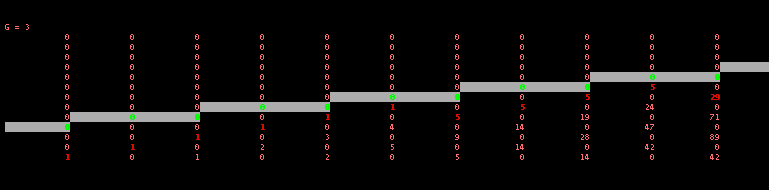
\includegraphics[scale=0.5]{photo.png}










<<<<<<< HEAD
%Take a look at each new configuration from $g$ starting at one to any finite, positive integer. Begin numbering the 
%diagonals of a corridor, starting at zero, for each configuration of $g$. The number of repeating diagonals present depends on 
%the value chosen for $n$. If one compares the diagonals between subsequent $g corridors$ with $g$ starting at $1$ to some 
%other natural number, geometric series of degree $diagonal number$ seem to form. 
=======
%Take a look at each new configuration from $g$ starting at one to any finite, positive integer. Begin numbering the diagonals of a corridor, starting at zero, for each configuration of $g$. The number of repeating diagonals present depends on 
%the value chosen for $n$. If one compares the diagonals between subsequent $g corridors$ with $g$ starting at $1$ to some other natural number, geometric series of degree $diagonal number$ seem to form. 
>>>>>>> 1c694aeb9381e22897e1cb9b8624807d72e6f7e3


% Even with the position of the starting value being fixed, the results are different with each unique value of $g$. One can 
%observe the interesting patterns that occur with each new configuration. What types of patterns, if any, exist when the 
% starting position is a point other than $(0,1)$? How can the ripple effects from differing values of $a$ be observed an analyzed?


%\subsection{chaning start position}
%\subsection{chagning slope}
%\subsection{with both changed}
%\subsection{changing start value}
%\subsection{all of the ripples happening section?}
%\subsection{conclusion and insightful remarks}
 \subsection*{Bibliography}
 %d;flsd;flk ~\cite{BanderierFlajolet}
 going to reference these\\*
 Shaun Ault and Charles Kicey Counting Lattice Paths Using Fourier Methods\\*
 Kenneth H. Rosen Discrete Mathematics and Its Applications\\*
 Richard A. Brualdi Introductory Combinatorics\\*
 C. Krattenthaller The Major Counting of Nonintersecting Lattice Paths and Generating Functions for Tableaux\\*
 Ting Kuo From Enumerating to Generating: A Linear Time Algorithm for Generating 2D Lattice Paths with a Given Number of Turns
 %\bibliography{test.bbl}{}
 %\bibliographystyle{plain}

 %*is there some special math format for citations? need to look that up maybe* \\*
 %used Dr. A and Dr. K paper \\*
 %used OIES get specific stuff used\\*
 %used library book jot down author name and info and other srcs \\*
\end{comment}

%w00t
\end{document}
